\graphicspath{{main/chapter1/fig/}}

\chapter{Context and Objectives}

% \vspace*{\fill}
\minitoccustom
% \vspace*{\fill}

\section{Introduction}

\begin{itemize}
  \item Shannon~\cite{Shannon1948}: système de communication (source -> émetteur
    -> canal -> récepteur -> destination)
  \item utilisé partout dans notre monde (télé, téléphone, internet, satellites,
    etc.)
  \item zoom sur l'émetteur (source -> codage canal -> modulation)
  \item zoom sur le récepteur (démodulation -> décodage canal -> destination)
  \item introduction au codage canal, nécessaire pour mieux résister aux
    perturbations dues à la traversée du signal dans un environnement physique
    (le canal)
  \item modulation: représentation d'une information numérique en analogique
    adaptée au canal
  \item évoquer la synchro avant la démodulation
  \item couche physique (PHY 1) du modèle OSI
  \item couche physique traditionnellement implémentée en hardware (ASIC)
  \item récepteur gourmand en calcul (plus particulière l'algorithme de décodage
    et un peu la démodulation)
\end{itemize}

It is now commonplace to state that Humanity has entered the era of
communication. Moreover, all kinds of objects will increasingly also use
communication technology, to exchange information in the \emph{Internet of
Things} (IoT). Despite their variety, all communication systems are based on a
common abstract model proposed by Claude Shannon. In his seminal
paper~\cite{Shannon1948}, he proposed to model a communication system with five
components: an information source, a transmitter, a channel, a receiver and a
destination. This model was later refined as shown in
Figure~\ref{fig:intro_com_chain}. The source produces a digital message to be
transmitted. The channel encoder transforms it to make it less prone to errors.
The modulator translates digital data into a physical signal. The channel alters
the signal with some noise and distortions. On the receiver side, the components
perform the inverse operations to retrieve the message produced by the source.

\begin{figure}[htp]
  \centering
  \begin{scaletikzpicturetowidth}{0.70\linewidth}
  \documentclass[tikz]{standalone}

\usepackage[T1]{fontenc}
\usepackage[utf8]{inputenc}
\usepackage{eulervm}
\usepackage{amsmath}
\usepackage{bm}
\usepackage{tikz}
\usepackage{environ}

\usetikzlibrary{fit}
\usetikzlibrary{patterns}
\usetikzlibrary{arrows}

\usepackage{color}

\definecolor{Comment}{RGB}{97,161,176}

\definecolor{btfGreen}{RGB}{51,160,44}
\definecolor{btfRed}{RGB}{190,60,90}

\definecolor{bleuUni}{RGB}{0, 157, 224}
\definecolor{marronUni}{RGB}{68, 58, 49}
\definecolor{grayMarronUni}{RGB}{60, 60, 60}
\definecolor{grayBleuUni}{RGB}{118, 118, 118}

\definecolor{bluecite}{HTML}{009DE0}

\definecolor{Paired-2}{RGB}{166,206,227}
\definecolor{Paired-1}{RGB}{31,120,180}
\definecolor{Paired-4}{RGB}{178,223,138}
\definecolor{Paired-3}{RGB}{51,160,44}
\definecolor{Paired-6}{RGB}{251,154,153}
\definecolor{Paired-5}{RGB}{227,26,28}
\definecolor{Paired-8}{RGB}{253,191,111}
\definecolor{Paired-7}{RGB}{255,127,0}
\definecolor{Paired-10}{RGB}{202,178,214}
\definecolor{Paired-9}{RGB}{106,61,154}
\definecolor{Paired-12}{RGB}{255,255,153}
\definecolor{Paired-11}{RGB}{177,89,40}
\definecolor{Accent-1}{RGB}{127,201,127}
\definecolor{Accent-2}{RGB}{190,174,212}
\definecolor{Accent-3}{RGB}{253,192,134}
\definecolor{Accent-4}{RGB}{255,255,153}
\definecolor{Accent-5}{RGB}{56,108,176}
\definecolor{Accent-6}{RGB}{240,2,127}
\definecolor{Accent-7}{RGB}{191,91,23}
\definecolor{Accent-8}{RGB}{102,102,102}
\definecolor{Spectral-1}{RGB}{158,1,66}
\definecolor{Spectral-2}{RGB}{213,62,79}
\definecolor{Spectral-3}{RGB}{244,109,67}
\definecolor{Spectral-4}{RGB}{253,174,97}
\definecolor{Spectral-5}{RGB}{254,224,139}
\definecolor{Spectral-6}{RGB}{255,255,191}
\definecolor{Spectral-7}{RGB}{230,245,152}
\definecolor{Spectral-8}{RGB}{171,221,164}
\definecolor{Spectral-9}{RGB}{102,194,165}
\definecolor{Spectral-10}{RGB}{50,136,189}
\definecolor{Spectral-11}{RGB}{94,79,162}
\definecolor{Set1-1}{RGB}{228,26,28}
\definecolor{Set1-2}{RGB}{55,126,184}
\definecolor{Set1-3}{RGB}{77,175,74}
\definecolor{Set1-4}{RGB}{152,78,163}
\definecolor{Set1-5}{RGB}{255,127,0}
\definecolor{Set1-6}{RGB}{255,255,51}
\definecolor{Set1-7}{RGB}{166,86,40}
\definecolor{Set1-8}{RGB}{247,129,191}
\definecolor{Set1-9}{RGB}{153,153,153}
\definecolor{Set2-1}{RGB}{102,194,165}
\definecolor{Set2-2}{RGB}{252,141,98}
\definecolor{Set2-3}{RGB}{141,160,203}
\definecolor{Set2-4}{RGB}{231,138,195}
\definecolor{Set2-5}{RGB}{166,216,84}
\definecolor{Set2-6}{RGB}{255,217,47}
\definecolor{Set2-7}{RGB}{229,196,148}
\definecolor{Set2-8}{RGB}{179,179,179}
\definecolor{Dark2-1}{RGB}{27,158,119}
\definecolor{Dark2-2}{RGB}{217,95,2}
\definecolor{Dark2-3}{RGB}{117,112,179}
\definecolor{Dark2-4}{RGB}{231,41,138}
\definecolor{Dark2-5}{RGB}{102,166,30}
\definecolor{Dark2-6}{RGB}{230,171,2}
\definecolor{Dark2-7}{RGB}{166,118,29}
\definecolor{Dark2-8}{RGB}{102,102,102}
\definecolor{Reds-1}{RGB}{255,245,240}
\definecolor{Reds-2}{RGB}{254,224,210}
\definecolor{Reds-3}{RGB}{252,187,161}
\definecolor{Reds-4}{RGB}{252,146,114}
\definecolor{Reds-5}{RGB}{251,106,74}
\definecolor{Reds-6}{RGB}{239,59,44}
\definecolor{Reds-7}{RGB}{203,24,29}
\definecolor{Reds-8}{RGB}{165,15,21}
\definecolor{Reds-9}{RGB}{103,0,13}
\definecolor{Greens-1}{RGB}{247,252,245}
\definecolor{Greens-2}{RGB}{229,245,224}
\definecolor{Greens-3}{RGB}{199,233,192}
\definecolor{Greens-4}{RGB}{161,217,155}
\definecolor{Greens-5}{RGB}{116,196,118}
\definecolor{Greens-6}{RGB}{65,171,93}
\definecolor{Greens-7}{RGB}{35,139,69}
\definecolor{Greens-8}{RGB}{0,109,44}
\definecolor{Greens-9}{RGB}{0,68,27}
\definecolor{Blues-1}{RGB}{247,251,255}
\definecolor{Blues-2}{RGB}{222,235,247}
\definecolor{Blues-3}{RGB}{198,219,239}
\definecolor{Blues-4}{RGB}{158,202,225}
\definecolor{Blues-5}{RGB}{107,174,214}
\definecolor{Blues-6}{RGB}{66,146,198}
\definecolor{Blues-7}{RGB}{33,113,181}
\definecolor{Blues-8}{RGB}{8,81,156}
\definecolor{Blues-9}{RGB}{8,48,107}


\begin{document}
  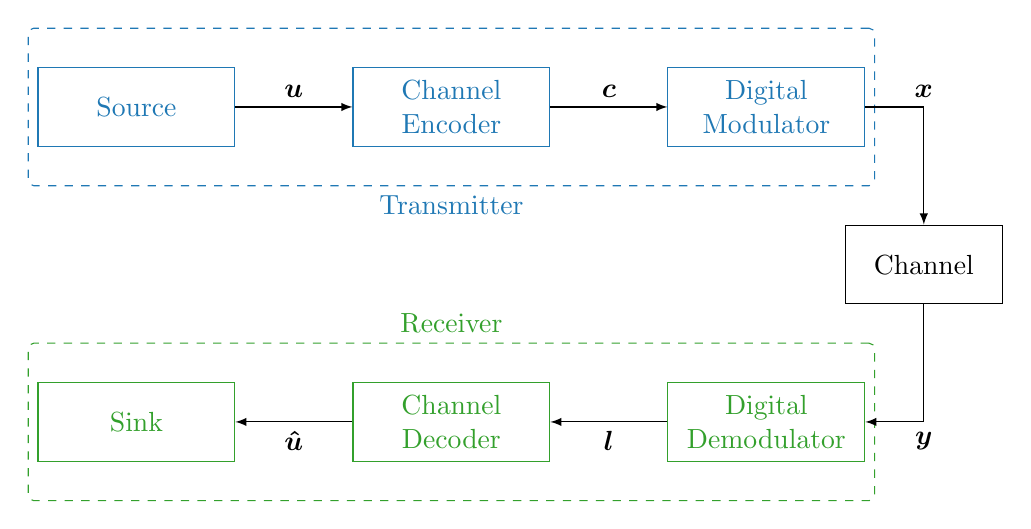
\begin{tikzpicture}%[scale=\tikzscale]
    \node[draw=Paired-1, rounded corners=0pt, minimum height=1cm, minimum width=2.5cm, text=Paired-1              ] (src) at ( 0, 4) {Source};
    \node[draw=Paired-1, rounded corners=0pt, minimum height=1cm, minimum width=2.5cm, text=Paired-1, align=center] (enc) at ( 4, 4) {Channel\\Encoder};
    \node[draw=Paired-1, rounded corners=0pt, minimum height=1cm, minimum width=2.5cm, text=Paired-1, align=center] (mod) at ( 8, 4) {Digital\\Modulator};
    \node[draw,          rounded corners=0pt, minimum height=1cm, minimum width=2.0cm,                            ] (chn) at (10, 2) {Channel};
    \node[draw=Paired-3, rounded corners=0pt, minimum height=1cm, minimum width=2.5cm, text=Paired-3, align=center] (dem) at ( 8, 0) {Digital\\Demodulator};
    \node[draw=Paired-3, rounded corners=0pt, minimum height=1cm, minimum width=2.5cm, text=Paired-3, align=center] (dec) at ( 4, 0) {Channel\\Decoder};
    \node[draw=Paired-3, rounded corners=0pt, minimum height=1cm, minimum width=2.5cm, text=Paired-3              ] (snk) at ( 0, 0) {Sink};

    \node[draw=Paired-1, rounded corners=2pt, label={[Paired-1]below:Transmitter}, minimum height=2cm, dashed, fit=(src) (enc) (mod)] {};
    \node[draw=Paired-3, rounded corners=2pt, label={[Paired-3]above:Receiver   }, minimum height=2cm, dashed, fit=(dem) (dec) (snk)] {};

    \draw[->,>=latex] (src) -- (enc) node [midway, above] {$\bm{u}$};
    \draw[->,>=latex] (enc) -- (mod) node [midway, above] {$\bm{c}$};
    \draw[->,>=latex] (mod) -| (chn) node [midway, above] {$\bm{x}$};
    \draw[->,>=latex] (chn) |- (dem) node [midway, below] {$\bm{y}$};
    \draw[->,>=latex] (dem) -- (dec) node [midway, below] {$\bm{l}$};
    \draw[->,>=latex] (dec) -- (snk) node [midway, below] {$\bm{\hat{u}}$};
  \end{tikzpicture}
\end{document}
  \end{scaletikzpicturetowidth}
  \caption{Digital communication chain.}
  \label{fig:intro_com_chain}
\end{figure}

The performance of this chain is measured by estimating the residual error rate
at the sink. This rate is directly driven by the choice of the channel encoder
and decoder. After Shannon, researchers have designed new coding/decoding
schemes to approach Shannon's theoretical limit ever closer. Indeed, recent
progresses managed to design practical codings performing very close to that
limit, and already integrated in everyday communication systems.

On the eve of the 5G mobile communication generation, the challenge is now to
design communication systems able to transmit huge amounts of data in a short
time, at a small energy cost, in a wide variety of environments. Researchers
work at refining existing coding schemes further, to get low residual error
rates with fast, flexible, low complexity decoders.

The validation of a coding scheme requires estimating its error rate
performance. Usually, no simple mathematical model exists to predict such
performance. The only practical solution is to perform a Monte Carlo simulation
of the whole chain: some data are randomly generated, encoded, modulated,
noised, decoded, and the performance is then estimated by measuring the Bit
Error Rate (BER) and the Frame Error Rate (FER) at the sink. This process leads
to three main problems:

\begin{enumerate}
  \item \textbf{Simulation time:}
    100 erroneous frames must be simulated to accurately estimate the FER/BER.
    Thus, measuring a FER of $10^{-7}$ requires simulating the transmission of
    $\sim100\times 10^7=10^9$ frames. Assuming a frame of 1000~bits, the
    simulator must then emulate the transmission of $10^{12}$~bits. Keeping in
    mind that the decoding algorithm complexity may be significant, several
    weeks or months may be required to accurately estimate the FER/BER of a
    coding scheme.

  \item \textbf{Algorithmic heterogeneity:} A large number of channel codes have
    been designed over time. For each kind of code, several decoding algorithms
    are available. While it is straightforward to describe a unique coding
    scheme, it is more challenging to have a unified software description that
    supports all the coding schemes and their associated algorithms. This
    difficulty comes from the heterogeneity of the data structure necessary to
    describe a channel code and the associated decoder: turbo codes use
    trellises, LDPC codes are well-defined on factor graphs and polar codes are
    efficiently decoded using binary trees.

  \item \textbf{Reproducibility:} It is usually tedious to reproduce results
    from the literature. This can be explained by the large amount of empirical
    parameters necessary to define one communication system, and the fact that
    not all of them are always reported in publications. Moreover, the simulator
    source codes are rarely publicly available. Consequently, a large amount of
    time is spent ``reinventing the wheel'' just to be able to compare to the
    state-of-the-art results.
\end{enumerate}

The long simulation times make it desirable to have \textbf{high throughput
implementations}. The algorithmic heterogeneity requires \textbf{flexible,
modular software}. The reproducibility issue pushes towards a \textbf{portable}
and \textbf{open-source software}. These are the purposes of \AFFECT.

\section{Channel Coding}

\begin{itemize}
  \item 3 grandes familles de code approchent la capacité du canal (limite de
    Shannon) : LDPC, Polar et Turbo, les décrire et les comparer
\end{itemize}

\subsection{Channel Models}

\begin{itemize}
  \item présenter modèles de canal (BEC, BSC, AWGN)
  \item introduire LLRs
\end{itemize}

\subsection{LDPC codes}

\subsection{Turbo codes}

\subsection{Polar codes}

\section{Simulation}

\begin{itemize}
  \item besoin d'implémentations logicielles pour estimer les performances des
    algorithmes de décodage avant de les implémenter en hardware (Monte-Carlo
    sur canal AWGN)
  \item Introduire BE, FE, BER, FER
\end{itemize}

\begin{figure}[htp]
  \centering
  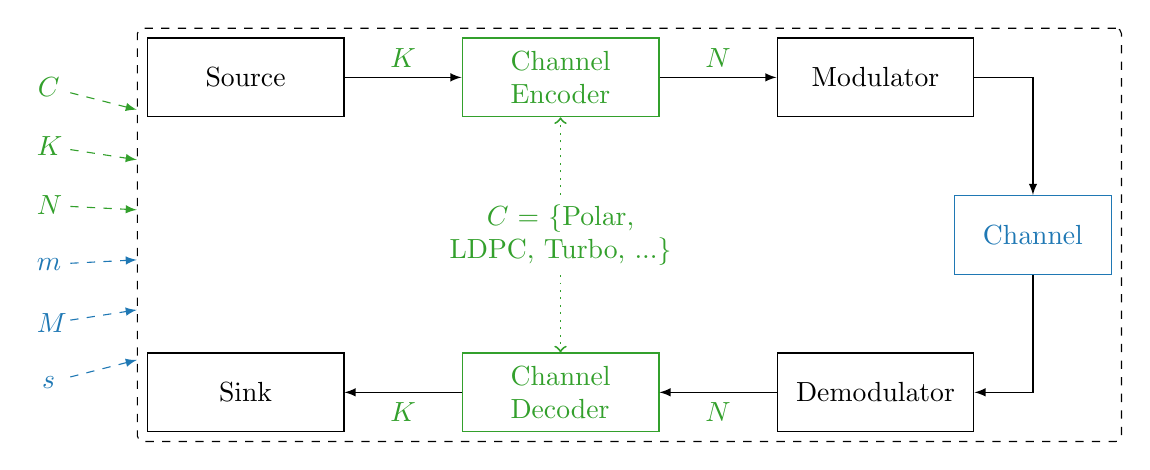
\begin{tikzpicture}
  \node[draw=black,    rounded corners=0pt, minimum height=1cm, minimum width=2.5cm, text=black               ] (src) at ( 0, 4) {Source};
  \node[draw=Paired-3, rounded corners=0pt, minimum height=1cm, minimum width=2.5cm, text=Paired-3, align=left] (enc) at ( 4, 4) {Channel\\Encoder};
  \node[draw=black,    rounded corners=0pt, minimum height=1cm, minimum width=2.5cm, text=black               ] (mod) at ( 8, 4) {Modulator};
  \node[draw=Paired-1, rounded corners=0pt, minimum height=1cm, minimum width=2.0cm, text=Paired-1            ] (chn) at (10, 2) {Channel};
  \node[draw=black,    rounded corners=0pt, minimum height=1cm, minimum width=2.5cm, text=black               ] (dem) at ( 8, 0) {Demodulator};
  \node[draw=Paired-3, rounded corners=0pt, minimum height=1cm, minimum width=2.5cm, text=Paired-3, align=left] (dec) at ( 4, 0) {Channel\\Decoder};
  \node[draw=black,    rounded corners=0pt, minimum height=1cm, minimum width=2.5cm, text=black               ] (snk) at ( 0, 0) {Sink};

  \draw[->,>=latex] (src) -- (enc) node [midway, above, fill=white, text=Paired-3] {$K$};
  \draw[->,>=latex] (enc) -- (mod) node [midway, above, fill=white, text=Paired-3] {$N$};
  \draw[->,>=latex] (mod) -| (chn) node [midway, above, fill=white               ] {};
  \draw[->,>=latex] (chn) |- (dem) node [midway, below, fill=white               ] {};
  \draw[->,>=latex] (dem) -- (dec) node [midway, below, fill=white, text=Paired-3] {$N$};
  \draw[->,>=latex] (dec) -- (snk) node [midway, below, fill=white, text=Paired-3] {$K$};

  \node[draw=black, rounded corners=2pt, minimum height=2cm, dashed, fit=(src) (enc) (mod) (chn) (dem) (dec) (snk)] (sim) {};

  \node[text width=0.3cm, text centered, text=Paired-3] (C) at (-2.5, 3.875) {$C$};
  \node[text width=0.3cm, text centered, text=Paired-3] (K) at (-2.5, 3.125) {$K$};
  \node[text width=0.3cm, text centered, text=Paired-3] (N) at (-2.5, 2.375) {$N$};
  \node[text width=0.3cm, text centered, text=Paired-1] (m) at (-2.5, 1.625) {$m$};
  \node[text width=0.3cm, text centered, text=Paired-1] (M) at (-2.5, 0.875) {$M$};
  \node[text width=0.3cm, text centered, text=Paired-1] (s) at (-2.5, 0.125) {$s$};

  \draw[->,>=latex, dashed, Paired-3] (C) -- (sim);
  \draw[->,>=latex, dashed, Paired-3] (K) -- (sim);
  \draw[->,>=latex, dashed, Paired-3] (N) -- (sim);
  \draw[->,>=latex, dashed, Paired-1] (m) -- (sim);
  \draw[->,>=latex, dashed, Paired-1] (M) -- (sim);
  \draw[->,>=latex, dashed, Paired-1] (s) -- (sim);

  \node[text width=4cm, text centered, text=Paired-3] (C2) at (4, 2) {$C$ = \{Polar, LDPC, Turbo, ...\}};

  \draw[->, dotted, Paired-3, line width=0.7pt] (C2) -- (enc);
  \draw[->, dotted, Paired-3, line width=0.7pt] (C2) -- (dec);
\end{tikzpicture}
  \caption{Main simulation parameters.}
  \label{fig:simu_com_chain}
\end{figure}

\begin{figure}[htp]
  \centering
  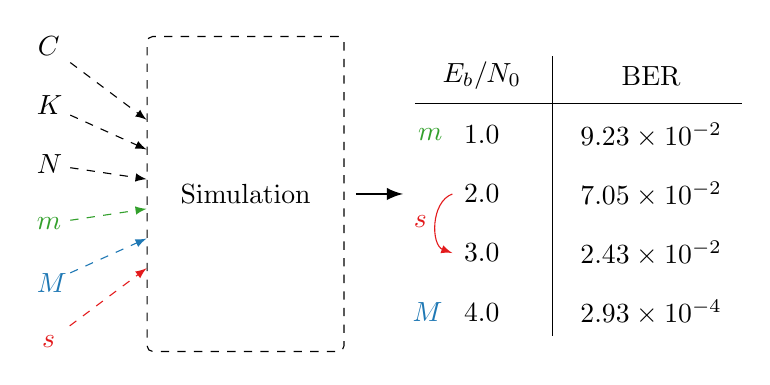
\begin{tikzpicture}%[scale=\tikzscale]
  \node[draw=black, rounded corners=2pt, minimum height=4cm, minimum width=2.5cm, text=black, dashed] (sim) at (0, 2) {Simulation};

  \node[text width=0.3cm, text centered, text=black   ] (C) at (-2.5, 3.875) {$C$};
  \node[text width=0.3cm, text centered, text=black   ] (K) at (-2.5, 3.125) {$K$};
  \node[text width=0.3cm, text centered, text=black   ] (N) at (-2.5, 2.375) {$N$};
  \node[text width=0.3cm, text centered, text=Paired-3] (m) at (-2.5, 1.625) {$m$};
  \node[text width=0.3cm, text centered, text=Paired-1] (M) at (-2.5, 0.875) {$M$};
  \node[text width=0.3cm, text centered, text=Paired-5] (s) at (-2.5, 0.125) {$s$};

  \draw[->,>=latex, dashed, black   ] (C) -- (sim);
  \draw[->,>=latex, dashed, black   ] (K) -- (sim);
  \draw[->,>=latex, dashed, black   ] (N) -- (sim);
  \draw[->,>=latex, dashed, Paired-3] (m) -- (sim);
  \draw[->,>=latex, dashed, Paired-1] (M) -- (sim);
  \draw[->,>=latex, dashed, Paired-5] (s) -- (sim);

  \draw[->,>=latex, black, line width=1.0pt] (1.40, 2) -> (2.0, 2);

  \draw (2.15, 3.15) -- (6.30, 3.15);
  \draw (3.90, 3.75) -- (3.90, 0.20);

  \node[text width=1.5cm, text centered                            ] (SNR1) at (3, 3.50) {$E_b/N_0$};
  \node[text width=0.5cm, text centered, label={[Paired-3]left:$m$}] (SNR2) at (3, 2.75) {$1.0$};
  \node[text width=0.5cm, text centered                            ] (SNR3) at (3, 2.00) {$2.0$};
  \node[text width=0.5cm, text centered                            ] (SNR4) at (3, 1.25) {$3.0$};
  \node[text width=0.5cm, text centered, label={[Paired-1]left:$M$}] (SNR5) at (3, 0.50) {$4.0$};

  \draw[->,>=latex, Paired-5] (SNR3.west) to[bend right=70] (SNR4.west) node [left, yshift=0.4cm, xshift=-0.2cm] {$s$};

  \node[text width=2cm, text centered] (BER1) at (5.15, 3.50) {BER};
  \node[text width=2cm, text centered] (BER2) at (5.15, 2.75) {$9.23 \times 10^{-2}$};
  \node[text width=2cm, text centered] (BER3) at (5.15, 2.00) {$7.05 \times 10^{-2}$};
  \node[text width=2cm, text centered] (BER4) at (5.15, 1.25) {$2.43 \times 10^{-2}$};
  \node[text width=2cm, text centered] (BER5) at (5.15, 0.50) {$2.93 \times 10^{-4}$};
\end{tikzpicture}
  \caption{Input simulation parameters and output BER results.}
  \label{fig:intro_in_out}
\end{figure}

\begin{figure}[htp]
  \centering
  \subfloat[][Polar codes.]        {\includegraphics[width=0.30\textwidth]{simu/bfer/bfer_polar} \label{fig:intro_bfer_polar}}  \quad{}
  \subfloat[][LDPC codes.]         {\includegraphics[width=0.30\textwidth]{simu/bfer/bfer_ldpc}  \label{fig:intro_bfer_ldpc}}   \quad{}
  \subfloat[][Turbo codes.]        {\includegraphics[width=0.30\textwidth]{simu/bfer/bfer_turbo} \label{fig:intro_bfer_turbo}}  \\
  \subfloat[][Turbo product codes.]{\includegraphics[width=0.30\textwidth]{simu/bfer/bfer_tpc}   \label{fig:intro_bfer_tpc}}    \quad{}
  \subfloat[][BCH \& RS codes.]    {\includegraphics[width=0.30\textwidth]{simu/bfer/bfer_bch_rs}\label{fig:intro_bfer_bch_rs}} \quad{}
  \subfloat[][Convolutional codes.]{\includegraphics[width=0.30\textwidth]{simu/bfer/bfer_rsc}   \label{fig:intro_bfer_rsc}}
  \caption{\AFFECT simulation of various code families.}
  \label{fig:intro_bfer}
\end{figure}

\section{Base Station and Cloud-RAN}

\begin{itemize}
  \item besoin d'implémentations software pour gagner en flexibilité et réduire
    les coûts par rapport au hardware dans les stations de base par ex. (SDR)
\end{itemize}

\section{Software Defined Radio (SDR)}

\section{Objectives}

\begin{itemize}
  \item High Performance
  \item Portability
  \item Algorithmic Heterogeneity
  \item Code re-use, pour éviter de tout jeter à chaque nouvel algo
\end{itemize}
